% --
% signal processing

\chapter{Signal Processing and Feature Extraction}\label{sec:signal}
\thesisStateNew
This section describes how raw waveforms from audio files are processed and meaningful features for speech recognition extracted.
The feature extraction compresses and reduces the dimension of input data and therefore computational effort for neural networks.
Either raw audio samples are used directly as features for Wavenets, or Mel Frequency Cepstral Coefficients (MFCC) features are extracted for Convolutional Neural Networks (CNN).
The extraction of MFCC features is described in detail as well as enhancements with deltas and energy features and a suitable visual representation for them.
Further an efficient onset method is described to restrict the time interval of spoken key words. 

% --
% raw audio

\section{Raw Audio Waveforms}\label{sec:signal_raw}
\thesisStateRevised
\thesisStateNew
Physical acoustic waves can be recorded by microphones, translating mechanical vibrations to electrical signals. 
Those electrical signals are further stored in \emph{waveform files} or \emph{audio files} with a specific audio format, for example the \texttt{.wav} format.
Apart from any compression technique the most important storage details are the bit resolution, for example \SI{24}{\bit} floating point and the sample rate $f_s$. 
The sample rate defines, which frequency range of a continuous acoustic waveform can be stored in a discrete representation.
This is restricted by the Nyquist-Shannon sampling theorem, where the maximal frequency of the signal $f_{x_{max}}$ should not exceed the half of the sampling frequency: 
\begin{equation}\label{eq:signal_raw_nyquist}
  f_{x_{max}} < \frac{f_s}{2}
\end{equation}
to prevent aliasing effects.
That is the reason, why the compact disc (CD) format has a sampling frequency of \SI{44.1}{\kilo\hertz} resulting in a maximum signal frequency of \SI{22.05}{\kilo\hertz}, using the fact that humans do not hear above \SI{20}{\kilo\hertz} frequencies.
However it is also possible to go far beyond those \SI{44.1}{\kilo\hertz}, for instance used in telephone systems, where the sampling rate is \SI{8}{\kilo\hertz}.
It is possible to reduce the sampling rate, because voice does not need such a high sampling frequency to have sufficient quality and being understandable.
Music on the other hand requires a high sampling frequency for being enjoyable to listen to.

With the sampling frequency known, a discrete time signal of an audio recording $\bm{x} \in \R^n$ can be expressed in vector notation:
\begin{equation}\label{eq:signal_raw_x}
  \bm{x} = [x_1, x_2, \dots, x_n]^T
\end{equation}
with a total number of $n$ samples.
The recorded audio files provided in the speech command dataset \cite{Warden2018} used for the experiments in \rsec{exp}, are sampled with a sampling rate of \SI{16}{\kilo\hertz}, which is enough for human speech signals.
Further those recordings usually have a time duration of \SI{1}{\second}, apart from some individual shorter files.

For evaluation and visualization purpose, the author of this thesis recorded his own examples of the speech commands \{\enquote{left}, \enquote{right}, \enquote{up}, \enquote{down}, \enquote{go}\} with a simple consumer lavalier microphone.
Those showcase examples, shown in \rfig{signal_raw_showcase} in raw audio format, will be used to illustrate the whole feature extraction process in the following sections.
\begin{figure}[!ht]
  \centering
    \subfigure[left]{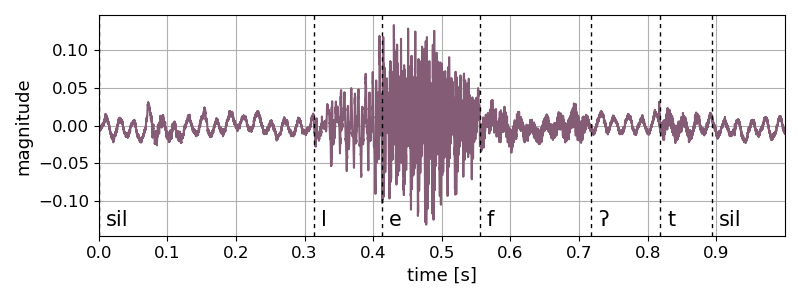
\includegraphics[width=0.45\textwidth]{./3_signal/figs/signal_raw_showcase_left0}}
    \subfigure[right]{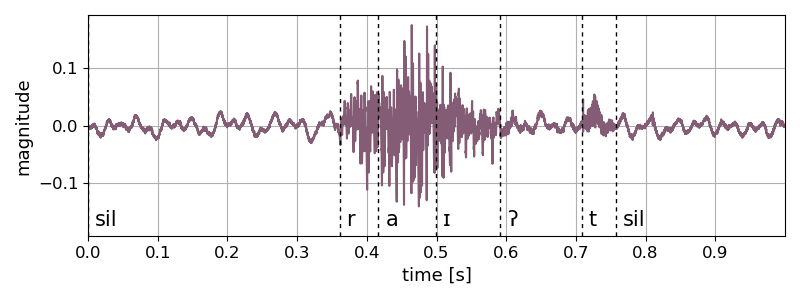
\includegraphics[width=0.45\textwidth]{./3_signal/figs/signal_raw_showcase_right0}}
    \subfigure[up]{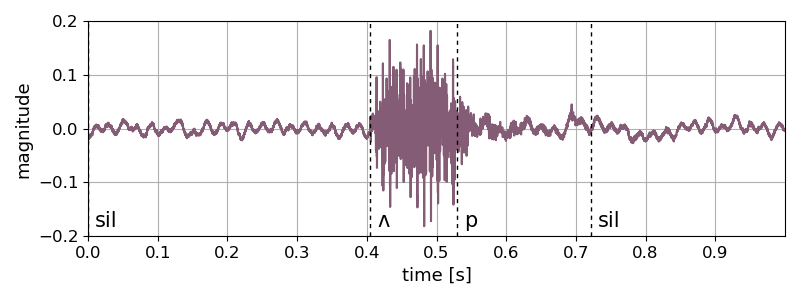
\includegraphics[width=0.45\textwidth]{./3_signal/figs/signal_raw_showcase_up0}}
    \subfigure[down]{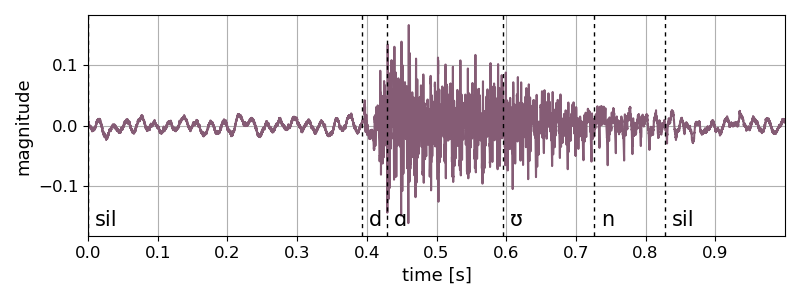
\includegraphics[width=0.45\textwidth]{./3_signal/figs/signal_raw_showcase_down0}}
    \subfigure[go]{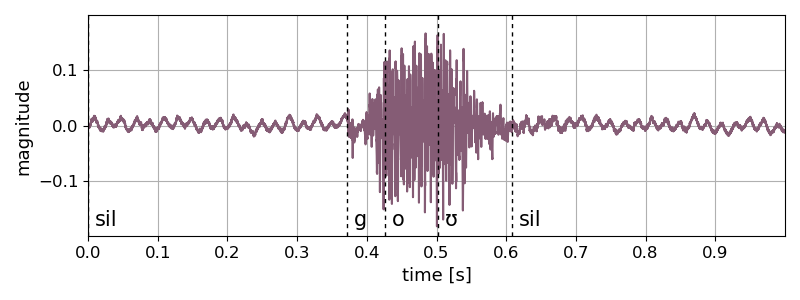
\includegraphics[width=0.45\textwidth]{./3_signal/figs/signal_raw_showcase_go0}}
  \caption{Self recorded raw audio waveform examples with phoneme onsets marked as vertical dashed lines.}
  \label{fig:signal_raw_showcase}
\end{figure}
\FloatBarrier
\noindent
From the shown raw audio files, it can be estimated how long a speech command may take in terms of duration and observed that usually \SI{1}{\second} is too much for a single speech command.
The pronunciation of words can of course deviate strongly in duration, but usually when commanding something it is preferred to speak short and well pronounced.
If a time interval of \SI{500}{\milli\second} is used to capture a speech command (this time interval is used in the feature extraction), it might happen that not every phoneme of the spoken words are captured. 
Often this might occur for words with glottal stops before consonants, for example the phoneme \enquote{t} in \enquote{left} or \enquote{right}, therefore the input features may only contain information of the first phonemes \enquote{lef} or \enquote{righ}.
But since Key Word Spotting (KWS) is restricted in its vocabulary and no similar words are contained within, it should be no problem in distinguishing those.

Another important aspect, when using limited time intervals for key words, is to detect an appropriate onset position (beginning of the key word) on the time axis of the signal.
It is easy to see in \rfig{signal_raw_showcase} where the spoken words are beginning and ending, but usually not all recordings are as clean as those.
There might be a large noise floor level, imminent background noise or cut off signals, so that the detection of the right onset position for the \SI{500}{\milli\second} time interval within the \SI{1}{\second} recordings is not always appropriate.
The onset detection is described separately in \rsec{signal_onset}.

At last it should be noted, that the value range in the y-axis of audio recordings strongly depends on the microphone, amplifiers and post processing.
It is therefore strongly recommended to normalize all recordings to a defined value range, achieved with for instance the infinity norm:
\begin{equation}
  \bm{x} \gets \frac{\bm{x}}{\norm{\bm{x}}_\infty}
\end{equation}
so that the maximum or minimum value of $\bm{x}$ corresponds to either $+1$ or $-1$ and the signal range is defined between $[-1, 1]$.
% --
% spectrogram

\section{Spectral Features}\label{sec:signal_spec}
\thesisStateRevised
Spectral features, such as a spectrogram, are the most intuitive form to represent audio waveforms. 
It is possible to observe active energy regions of certain frequency bands that are active at consecutive time chunks.
Methodically this is done by shifting an \emph{analytic window} of time span $t_N$, on the time axis.
The time shifting has also a fixed time interval, denoted as \emph{hop time} $t_{h}$.
Both time parameters $t_N$ and $t_h$ can also be presented in samples through a multiplication with the sampling frequency $f_s$:
% --
% samples
\begin{equation}
  \begin{split}
    N &= t_N \, f_s, \\
    h &= t_h \, f_s.
  \end{split}
\end{equation}
Note that by shifting an analytic window of size $N$ with hop size $h$ will create a new resolution on the time axis, denoted as \emph{frames}.
The audio samples contained by the analytic window of size $N$, are transformed with the Discrete Fourier Transform (DFT):
% --
% DTFT
\begin{equation}\label{eq:signal_spec_dtft}
  \hat{x}[k] = \sum_{n=0}^{N-1} x[n] \, e^{-j\frac{2 \pi n}{N}k}
\end{equation}
into the frequency space $\hat{x}[k] \in \C$ with frequency index $k$ and discrete audio samples $x[n]$ with sample index $n$.
More conveniently, \req{signal_spec_dtft} can be written in matrix notation with the DFT operator denoted as $\mathcal{F} \in \C^{K \times N}$ with a total number of $N$ samples of the input signal $\bm{x} \in \R^N$ and $K$ Fourier coefficients:
%--
% DFT matrix
\begin{equation}\label{eq:signal_spec_dtft_matrix}
  \hat{\bm{x}} = \mathcal{F} \bm{x} \quad \mathrm{with} 
  \quad \mathcal{F}[k, n] = e^{-j\frac{2 \pi n}{N} k},
  \quad n,\, k = (0, 1, \dots, N-1),\, (0, 1 \dots, K-1)
\end{equation}
where $k$ and $n$ are row and column indices in the transformation matrix $\mathcal{F}$, which gives an output dimension of the DFT transformed signal $\hat{\bm{x}} \in \C^K$.

The length of the analytic window in samples $N$ is crucial for the frequency resolution and the lowest frequency that can be represented.
For example, the periodic time of a sound with $f=\SI{20}{\hertz}$ is $t=\frac{1}{f} = \SI{50}{\milli\second}$.
To represent a waveform it is necessary to have at least a quarter of its wavelength captured.
Within this thesis, the length of the analytic window is selected to \SI{25}{\milli\second}, which is enough for speech signals.

The \emph{hop size} $h$ in samples of the hop time $t_h$, by which the analytical window is shifted on the time axis, indicates the resolution in time and is especially important for sequential changes within the audio data.
In applications like speech processing the hop time should be selected, so that the fastest pronounced phone and its transitions to other phones is captured with sufficient resolution.
Usually a hop time of $t_{h}=\SI{10}{\milli\second}$ is chosen for speech recognition tasks (also used within this thesis), but it could be extended to $t_{h}=\SI{20}{\milli\second}$, applied in \cite{Peter2020} to save computations.

With the hop size $h$ in samples and $N$ the length of the analytical window, the Short-Time Fourier Transform (STFT) for discrete time signals, can be computed as:
% --
% stft
\begin{equation}\label{eq:signal_spec_stft}
    \tilde{X}[m, k] = \sum_{n=0}^{N-1} x[n + m h] \, w[n] \, e^{-j\frac{2 \pi n}{N}k}, \qquad m = 0, 1, \dots, M
\end{equation}
so that $\tilde{X}[m, k] \in \C$ is the STFT coefficient of frame $m$ and DFT coefficient $k$, where $n$ is denoted here as summation index, $w$ as a window function, such as the \emph{Hanning} window, $m$ indicates the frame index shifted by the hop size $h$ and $M$ is the maximum number of frames.
% until the end of the signal is reached by shifting the analytical window of size $N$ by the hop size on the discrete time axis.
The maximum number of frames $M$ is the total number of shifts of an analytical window of size $N$ by the hop size $h$ and can therefore be computed as:
% --
% hop
\begin{equation}\label{eq:signal_spec_hop}
  M = \ceil*{\frac{n-N}{h}}
\end{equation}
where $n$ is here the length of the discrete time signal $x \in \R^n$.
The calculation of the STFT can be written in matrix notation if the input chunks from the shifting of the analytic window is denoted as vector:
\begin{equation}
  \bm{x}_m = [\, x_{m h}, \dots, x_{m h+N}]^T
\end{equation}
where each individual $\bm{x}_m \in \R^N$ can be concatenated in a matrix $X \in \R^{N \times M}$ denoted as:
\begin{equation}
  X = [\bm{x}_0,\, \bm{x}_1,\, \dots,\, \bm{x}_M]
  % X = 
  % \begin{bmatrix}
  %   \bar{x}_1^T \\
  %   \vdots\\
  %   \bar{x}_M^T \\
  % \end{bmatrix}
\end{equation}
so that the STFT $\tilde{X} \in \C^{K \times M}$ can be conveniently written as:
% --
% stft matrix
\begin{equation}\label{eq:signal_spec_stft_matrix}
  \tilde{X} = \mathcal{F} \, \diag{\bm{w}} \, X
\end{equation}
where $\diag{\bm{w}}$ is a diagonal matrix of weight vectors with a realization of a window function $\bm{w} \in \R^N$ in vector notation.
The matrix $\tilde{X} \in \C^{K \times M}$ represents the whole STFT where the rows represent the shifts of the analytical window on the time axis and the columns the Fourier coefficients of each DFT.
The used STFT parameters for this thesis are shown in \rtab{signal_spec_stft}.
% --
% stft params
% --
% stft params
\begin{table}[ht!]
\begin{center}
\caption{Parameters used for the STFT computation.}
\begin{tabular}{ M{4cm}  M{4cm}}
\toprule
\textbf{Parameter} & \textbf{Value} \\
\midrule
Sampling Frequency & \SI{16}{\kilo\hertz}\\
Analytic window size & \SI{25}{\milli\second}\\
Hop size & \SI{10}{\milli\second}\\
Window Function & Hanning\\
\bottomrule
\label{tab:signal_spec_stft}
\end{tabular}
\end{center}
\vspace{-4mm}
\end{table}
\FloatBarrier
\noindent
A spectrogram $P \in \R^{K \times M}$ is simply the power spectrum of the STFT $\tilde{X} \in \C^{K \times M}$ computed as:
% --
% spec
\begin{equation}\label{eq:signal_spec_spec}
  P = \abs{\tilde{X}}^2.
\end{equation}
Note that $P$ has now real values instead of complex ones.
The recorded examples transformed to a spectrogram with linear representation is shown in \rfig{signal_spec_lin_showcase}.
\begin{figure}[!ht]
  \centering
    \subfigure[left]{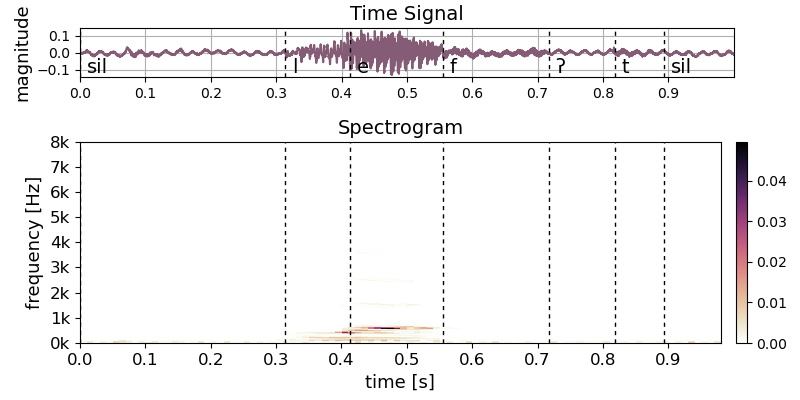
\includegraphics[width=0.45\textwidth]{./3_signal/figs/signal_spec-lin_showcase_left0}}
    \subfigure[right]{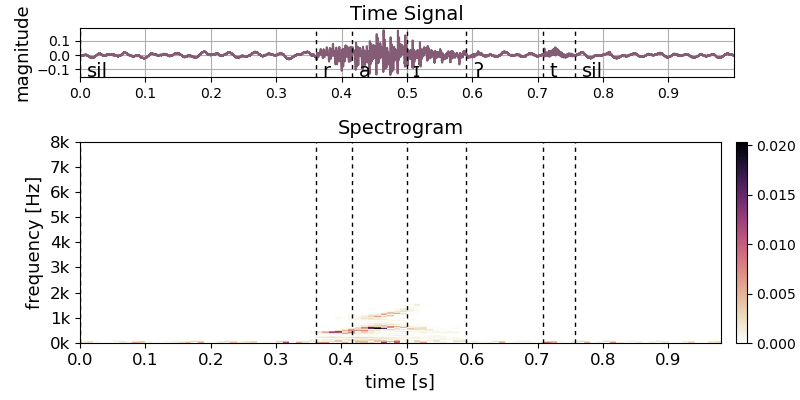
\includegraphics[width=0.45\textwidth]{./3_signal/figs/signal_spec-lin_showcase_right0}}
    \subfigure[up]{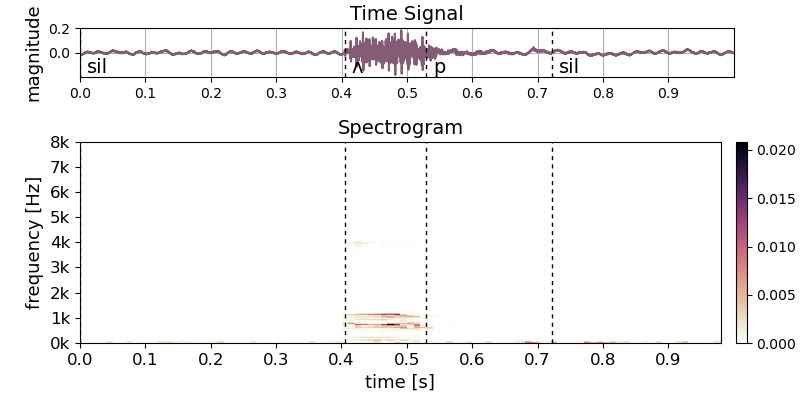
\includegraphics[width=0.45\textwidth]{./3_signal/figs/signal_spec-lin_showcase_up0}}
    \subfigure[down]{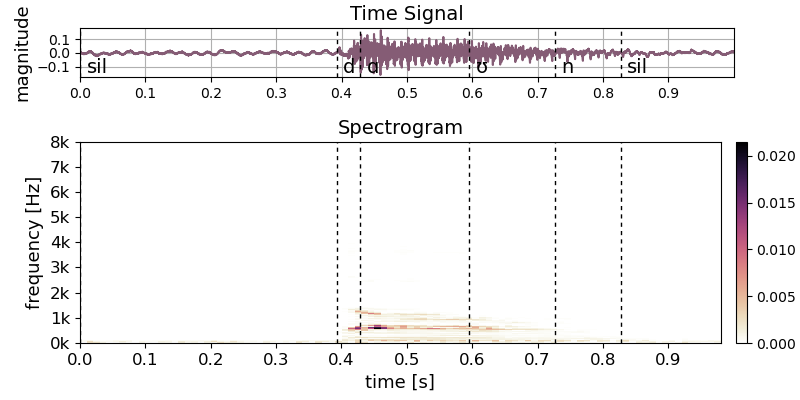
\includegraphics[width=0.45\textwidth]{./3_signal/figs/signal_spec-lin_showcase_down0}}
    \subfigure[go]{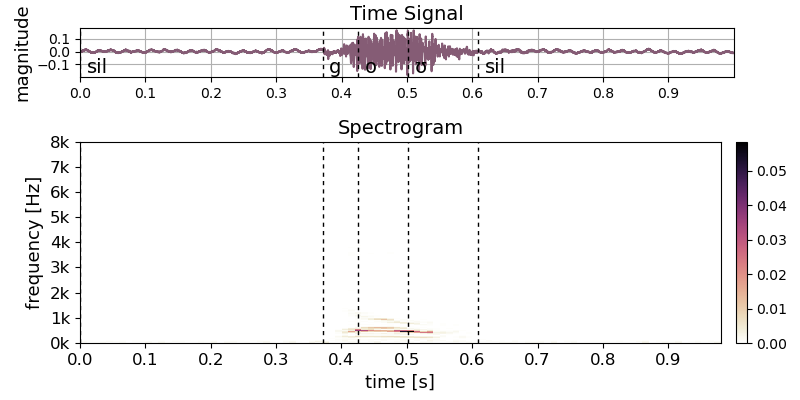
\includegraphics[width=0.45\textwidth]{./3_signal/figs/signal_spec-lin_showcase_go0}}
  \caption{Spectrogram linear scaled.}
  \label{fig:signal_spec_lin_showcase}
\end{figure}
\FloatBarrier
\noindent
It can be observed, that most of the signals energy is in the lower frequency regions of under approximately \SI{1}{\kilo\hertz}, therefore it is more appealing to transform the spectrogram into the log scale of its value space, achieved by:
% --
% log
\begin{equation}\label{eq:signal_spec_log}
  P_{DB} = 10 \cdot \log{P}
\end{equation}
so that small energies are more emphasized with $P_{DB} \in \R^{K \times M}$. 
The same examples with log scaling in the value space visualized with log scaling of the frequency space in the plots are shown in \rfig{signal_spec_log_showcase}.
\begin{figure}[!ht]
  \centering
    \subfigure[left]{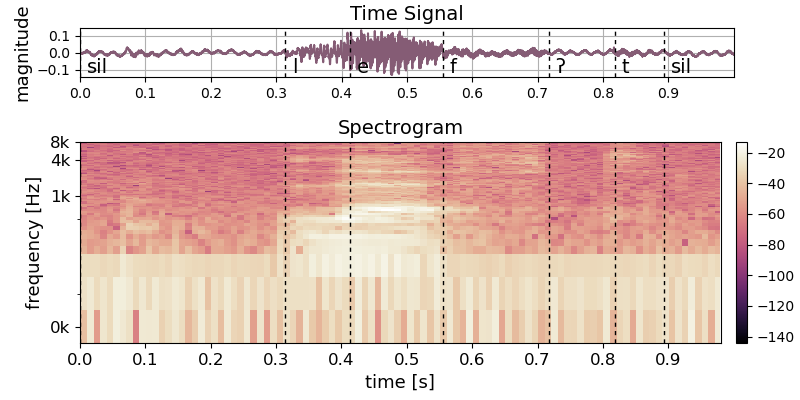
\includegraphics[width=0.45\textwidth]{./3_signal/figs/signal_spec-log_showcase_left0}}
    \subfigure[right]{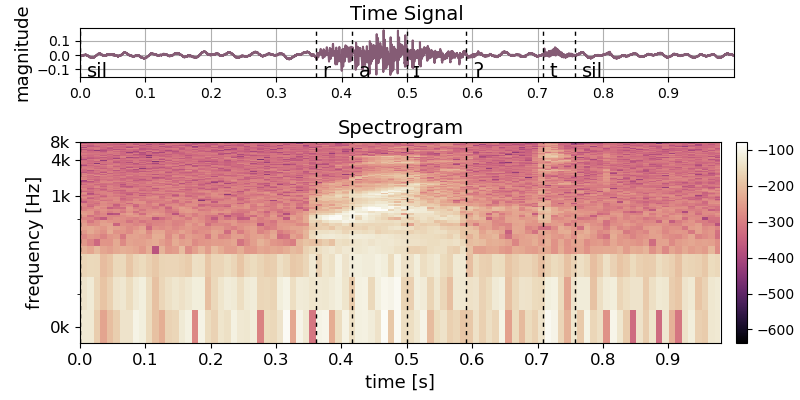
\includegraphics[width=0.45\textwidth]{./3_signal/figs/signal_spec-log_showcase_right0}}
    \subfigure[up]{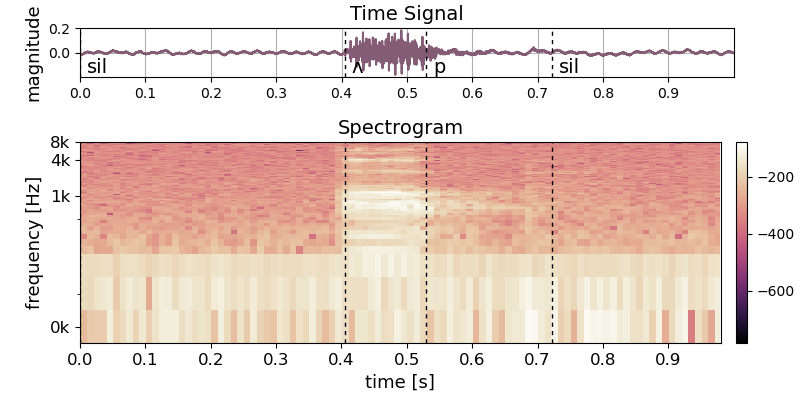
\includegraphics[width=0.45\textwidth]{./3_signal/figs/signal_spec-log_showcase_up0}}
    \subfigure[down]{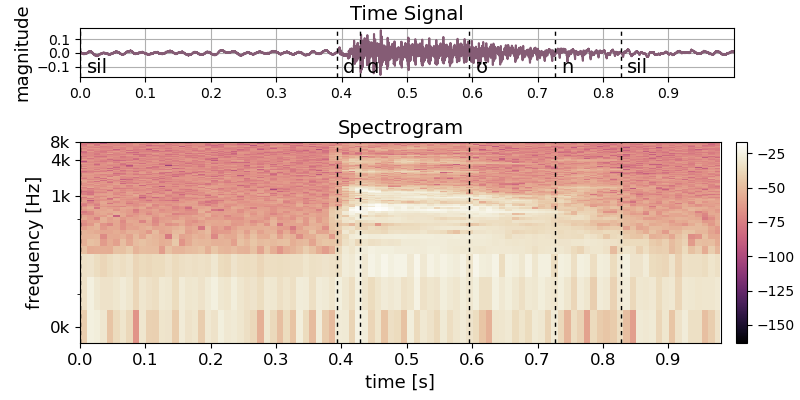
\includegraphics[width=0.45\textwidth]{./3_signal/figs/signal_spec-log_showcase_down0}}
    \subfigure[go]{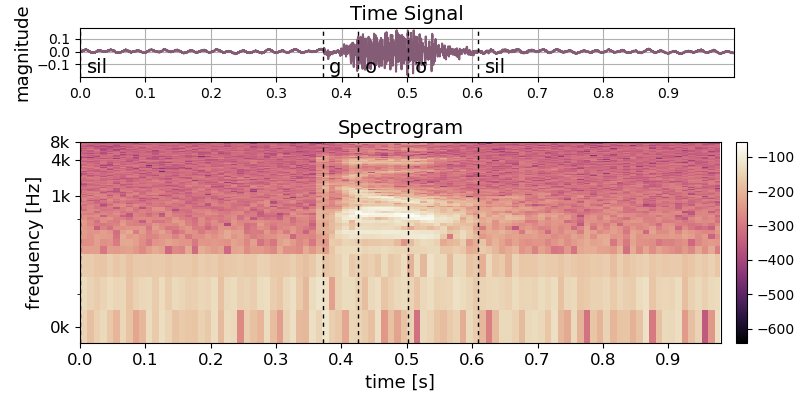
\includegraphics[width=0.45\textwidth]{./3_signal/figs/signal_spec-log_showcase_go0}}
  \caption{Spectrogram logarithmic scaled.}
  \label{fig:signal_spec_log_showcase}
\end{figure}
\FloatBarrier
\noindent
It is now possible to observe some interesting structures and movements in certain frequency bands over time.
A compression scheme, such as the Mel Frequency Cepstral Coefficients (MFCC) explained in the next section, reduces the high dimensional frequency feature vectors of the STFT to more compact feature vectors and further improves the visualization of the spoken command words.
% --
% mfcc

\section{Mel Frequency Cepstral Coefficients}\label{sec:signal_mfcc}
\thesisStateRevised
Very commonly Mel Frequency Cepstral Coefficients (MFCC) are used as input features for neural network classifications tasks in speech recognition.
It is described why MFCCs are good features for speech signals, how they are calculated in detail, how they can be enhanced and in which way they can be visualized to understand them better.


% --
% idea

\subsection{The Idea}
The processing scheme of MFCCs \cite{Mermelstein1980} is as following:
Raw audio samples are transformed into the frequency domain with the Short-Time Fourier Transform (STFT).
Afterwards the power spectrum of the STFT is segmented in frequency bands (along the frequency dimension) done by a filter bank.
The filter bands are spaced in equidistant Mel frequencies, where Mel frequencies represent the non-linear relationship between the Mel and frequency scale.
The Mel scale was developed in psycho-acoustic experiments, where researchers found out, that high frequency sounds (above approximately \SI{500}{\hertz}) are perceived lower than they actual are in the musical sense of pitch.
In the musical sense, a pitch interval of an octave is the doubling of the frequency of a fundamental frequency, but human hearing is different in the perception and frequency doubling does not necessarily double the perceived pitch.
As conclusion the Mel scale is suited human hearing perception of pitch and taking equidistant Mel bands is a reasonable approach.

Another important processing step is the logarithmic scaling of the power spectrum's value space, because humans perceive loudness in the logarithmic scale.
The last step is not that straight forward, but is a technique widely used in image processing called the Discrete Cosine Transform (DCT).
Note that the DCT is some kind of decorrelation process to mix filter bands in different constellations together.

This processing steps seem rather complicated, but are in fact nothing else but consecutive steps of appropriate scaling and data compression.
In fact neural networks are able to handle large amounts of input features, but it is always preferable to minimize the input size, hence the model size and training time are decreased and therefore computations saved.


% --
% processing pipeline

\subsection{Processing Pipeline in detail}\label{sec:signal_mfcc_pipeline}
The frequency spectrum is separated into filter bands through triangular window functions.
Those window functions are equidistantly placed onto the Mel scale and therefore give a varying number of frequency bins in the frequency scale of each window.
The lower frequency bands receive less frequency bins than the high frequency bands.
Sometimes the height of the triangular windows are scaled down so that the effect of unequal amounts frequency bin numbers is equalized, however high frequencies carry less energy and therefore this scaling is in most cases not needed, therefore all the triangular windows have their peak at the value $1$.
The Mel - Frequency relation can be approximated with:
% mel
\begin{equation}\label{eq:signal_mfcc_mel}
  m(f) = 2595 \cdot \log_{10} \left(1 + \frac{f}{700} \right) 
\end{equation}
where $m$ is the result in Mel scale as function of the frequency $f$.
The Mel scale plotted against the frequency scale is illustrated in \rfig{signal_mfcc_mel_scale}.
% mel fig
\begin{figure}[!ht]
  \centering
  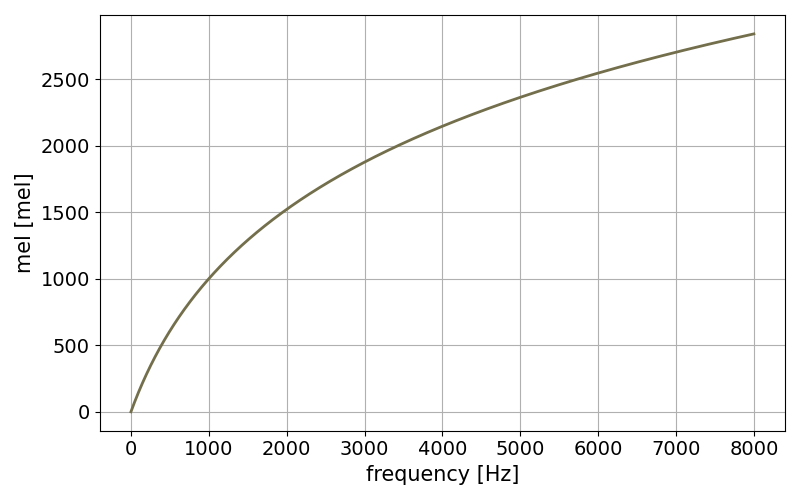
\includegraphics[width=0.40\textwidth]{./3_signal/figs/signal_mfcc_mel_scale}
  \caption{Mel scale as function of the frequency in a range of [0, \SI{16}{\kilo\hertz}].}
  \label{fig:signal_mfcc_mel_scale}
\end{figure}
\FloatBarrier
\noindent
The Mel and frequency window functions or equidistant Mel filter bands are shown in \rfig{filter_bands}.
\begin{figure}[!ht]
  \centering
  \subfigure[mel space]{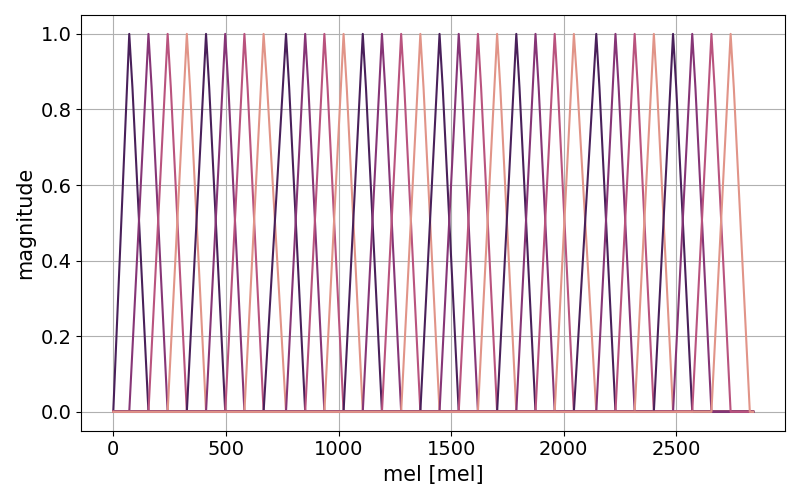
\includegraphics[width=0.40\textwidth]{./3_signal/figs/signal_mfcc_weights_mel}}
  \quad
  \subfigure[frequency space]{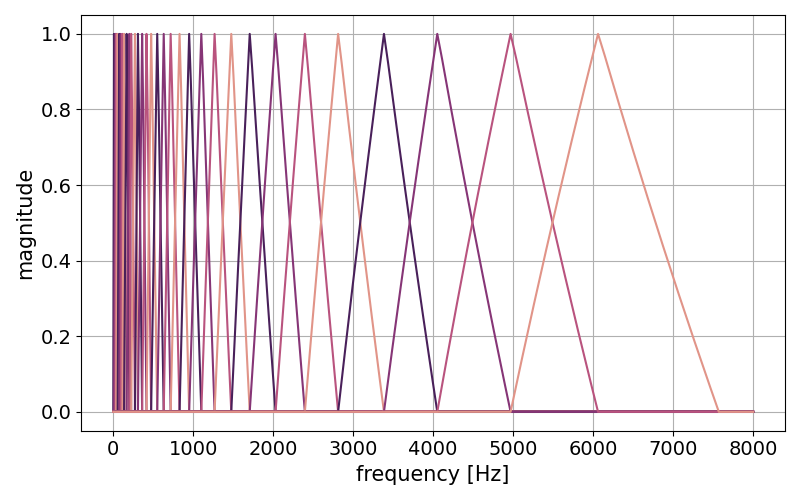
\includegraphics[width=0.40\textwidth]{./3_signal/figs/signal_mfcc_weights_f}}
  \caption{Equidistant Mel filter bands with a total number of 32 bands.}
  \label{fig:filter_bands}
\end{figure}
\FloatBarrier
\noindent
The creation of those filter bands is not described mathematically, because the graphical showcase is much more intuitive and easier to understand.
For further calculations, those filter bands are notated in a weight matrix called $W_m \in \R^{B \times N}$, where $B$ are the amount of used filter bands as rows in the matrix and $N$ the amount of frequency bins of the DFT transformed input signal as columns.

% dct
The DCT is very similar to the Fourier transform and projects the input signal to a set of orthogonal basis functions, however the transformed signal is real valued only instead of complex valued.
Different types of DCTs formulations exists, but most commonly the \enquote{type 2} DCT is used and can be calculated as:
% dct
\begin{equation}\label{eq:signal_mfcc_dct}
  X[c] = \sum_{n=0}^{N-1} x[n] \, \cos{\left[ \frac{\pi}{N} \left( n + \frac{1}{2} \right) c \right]}
\end{equation}
with $c$ as DCT coefficient index and $n$ as sample index of a signal with total length of $N$.
This can be conveniently written in matrix notation with a total number of $C$ DCT coefficients:
% dct matrix
\begin{equation}\label{eq:signal_mfcc_dct_matrix}
  X =  x^T \, \mathcal{D} \quad \mathrm{with} \quad \mathcal{D}[n, c] = \cos{\left[ \frac{\pi}{N} \left( n + \frac{1}{2} \right) c  \right]}, 
  \quad n, c = (0, 1 \dots N - 1), (0, 1 \dots C) 
\end{equation}
with $\mathcal{D} \in \R^{N \times C}$ as DCT matrix and input signal $x \in \R^N$ which gives the transformed signal $X \in \R^C$
The DCT basis functions illustrated in a matrix in two different color schemes are shown in \rfig{signal_mfcc_dct}.
\begin{figure}[!ht]
  \centering
  \subfigure[DCT with continuous color scheme]{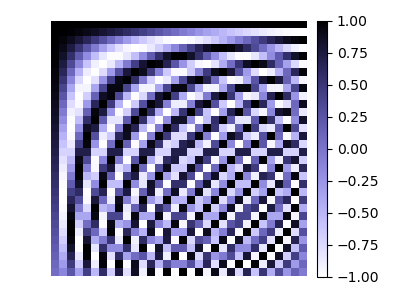
\includegraphics[width=0.35\textwidth]{./3_signal/figs/signal_mfcc_dct}}
  \quad
  \subfigure[DCT with diverging color scheme]{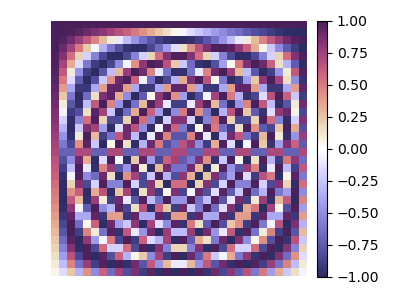
\includegraphics[width=0.35\textwidth]{./3_signal/figs/signal_mfcc_dct-div}}
  \caption{DCT matrix with 32 basis functions illustrated with a continuous and a diverging color scheme.}
  \label{fig:signal_mfcc_dct}
\end{figure}
\FloatBarrier
\noindent
The MFCCs $U \in \R^{M \times C}$ are calculated from the log scaled power spectrum of the STFT $\tilde{X} \in \C^{M \times K}$ computed in \req{signal_spec_stft_matrix}, the filter band weights collected in the matrix $W_m \in \R^{B \times K}$ and transformed with the DCT matrix $\mathcal{D} \in \R^{B \times C}$ as following:
\begin{equation}\label{eq:signal_mfcc_mfcc}
    U = \log{ \left[ \, \abs{\tilde{X}}^2 \, W_m^T \, \right] } \, \mathcal{D}.
\end{equation}
Note that the rows represent all shifts with the hop size and the columns are the individual cepstral coefficients of $U$.
The parameters to choose from are therefore the amount of filter bands $B$ and the amount of cepstral coefficients $C$.

Another important aspect is the visualization of MFCC features.
MFCCs computed as shown above, are not well intended for visualizations, because their individual coefficients value space differs strongly from each other.
For example the first coefficient equals a summation of all filter bands of the spectrogram and is therefore some kind of energy measure, while the other coefficients are different weighted sum combinations of the filter bands.
Further the most of the signal energy is located in the lower frequency bands, which impacts the value space of the coefficients with strongly weighted low frequency bands.
The differences in the value space leads to a problem in the visualization with a linear color scheme, so that some coefficients changes cannot be shown appropriately.
A solution to this problem is to normalize the feature vectors over each frame dimension with the infinity norm as:
% frame based normalization
\begin{equation}\label{eq:signal_mfcc_norm}
  \hat{U}[m, c] = \frac{U[m, c]}{\norm{u_c[m]}_\infty} \quad \forall \, m, c = (1, \dots, M), (1, \dots, C)
\end{equation}
where $m$ is again the frame (time) index, $c$ the individual MFCC coefficient and $u_c[m]$ the individual MFCC coefficient vector over all frames.
This equation gives a value space between $[0, 1]$ for each feature vector $u_c[m]$.

A visualization of MFCC features with 32 filter bands and 32 cepstral coefficients with frame based normalization of each coefficient is shown in \rfig{signal_mfcc_showcase_mfcc32}.
\begin{figure}[!ht]
  \centering
    \subfigure[left]{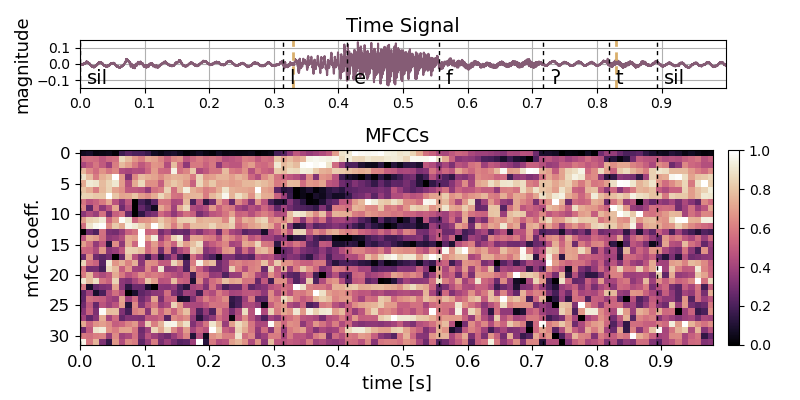
\includegraphics[width=0.45\textwidth]{./3_signal/figs/signal_mfcc_showcase_mfcc32_left0}}
    \subfigure[right]{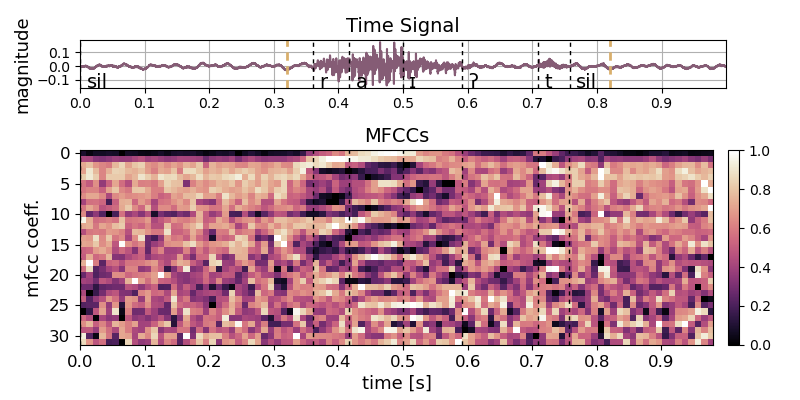
\includegraphics[width=0.45\textwidth]{./3_signal/figs/signal_mfcc_showcase_mfcc32_right0}}
    \subfigure[up]{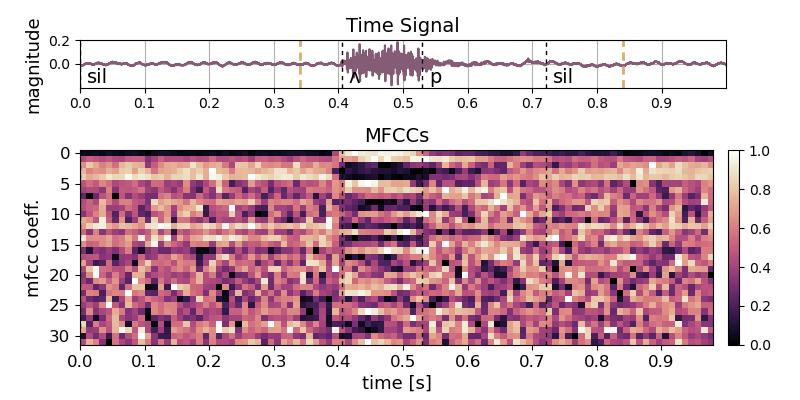
\includegraphics[width=0.45\textwidth]{./3_signal/figs/signal_mfcc_showcase_mfcc32_up0}}
    \subfigure[down]{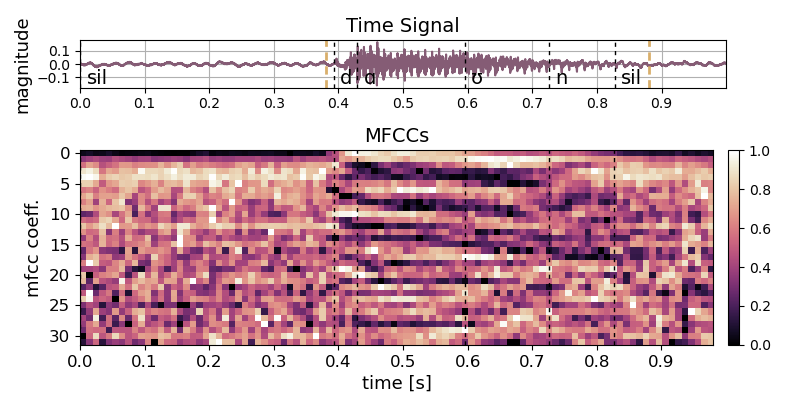
\includegraphics[width=0.45\textwidth]{./3_signal/figs/signal_mfcc_showcase_mfcc32_down0}}
    \subfigure[go]{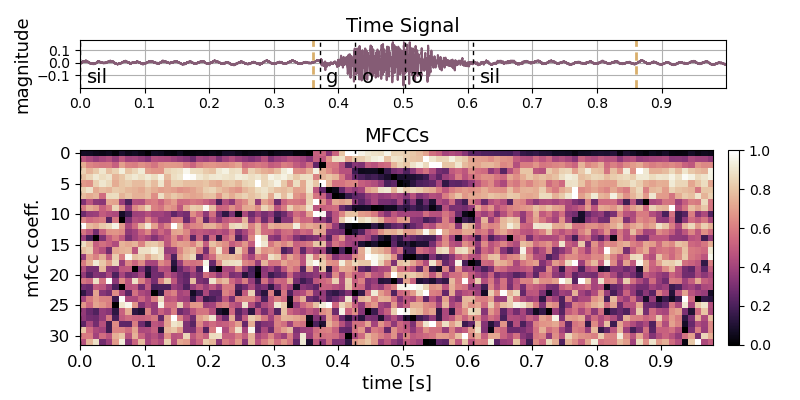
\includegraphics[width=0.45\textwidth]{./3_signal/figs/signal_mfcc_showcase_mfcc32_go0}}
  \caption{MFCC with 32 filter bands and 32 cepstral coefficients visualized with frame-based normalization.}
  \label{fig:signal_mfcc_showcase_mfcc32}
\end{figure}
\FloatBarrier
\noindent
The frame based normalization is an interesting aspect to improve the visualization of the MFCC features, however it can be critical. 
A normalization that operates only in one dimension changes important structures within the feature space and it cannot be answered yet if this is a problem for neural networks or degrades the classification performance.
One more research question arises here: Is it possible to use frame based normalized MFCC features as inputs to neural networks and what are the results to the accuracy and training of the models.


% --
% enhancement

\subsection{MFCC Feature Usage and Enhancement}\label{sec:signal_mfcc_enhancement}
After the MFCCs are computed with the choice of filter bands $B$ and cepstral coefficients $C$, they can already be used as input features for neural networks.
The question arises, whether feature enhancement can improve the performance in classification.
The best practice, applied in many papers, is to use $B=32$, $C=12$, compute derivatives of those 12 MFCC coefficients named as deltas (first derivative regarding the frame dimension) and double deltas (second derivative) and add energy vectors of the 12 coefficients and each one of the deltas.
The deltas are simply computed as frame $m$ difference of the MFCCs with:
\begin{equation}\label{eq:signal_mfcc_delta}
  \Delta u_i[m] = \frac{u_i[m - 1] + u_i[m + 1]}{2}
\end{equation}
where $u_i \in \R^M$ is the i-th MFCC coefficient vector and $m$ the frame index.
Note that the computation of the deltas at the edges $m=0$ and $m=M$ is not possible and the same value is obtained from the neighbor at this specific locations.
The second derivative of MFCC features, known as double deltas, are the frame differences of the deltas and in the same way computed as in \req{signal_mfcc_delta}.
Another enhancement is the computation of an energy feature vector of the MFCCs with:
\begin{equation}
  e[m] = u[m]^T \, u[m] 
\end{equation}
where $u[m] \in \R^C$ is the MFCC feature vector of frame $m$.
The same energy computation may also be applied to the deltas and double deltas each.
The MFCCs, their deltas, double deltas and energy vectors can simply be stacked at top of each other and used as enhanced feature inputs to neural networks.
In this thesis the feature vectors are stacked as following:
\begin{enumerate}
    \item 12 MFCCs
    \item 1 Energy feature of the 12 MFCCs
    \item 12 Deltas
    \item 1 Energy feature of the 12 Deltas
    \item 12 Double Deltas
    \item 1 Energy feature of the 12 Double Deltas
\end{enumerate}
which sums up to a 39-dimensional feature vector, very commonly used in the literature.
Many papers do not explicitly explain how the 39 MFCCs are calculated in detail, in most cases however this constellation is applied.
The computation of 39 MFCCs are shown in \rfig{signal_mfcc_showcase_mfcc39}
\begin{figure}[!ht]
  \centering
    \subfigure[left]{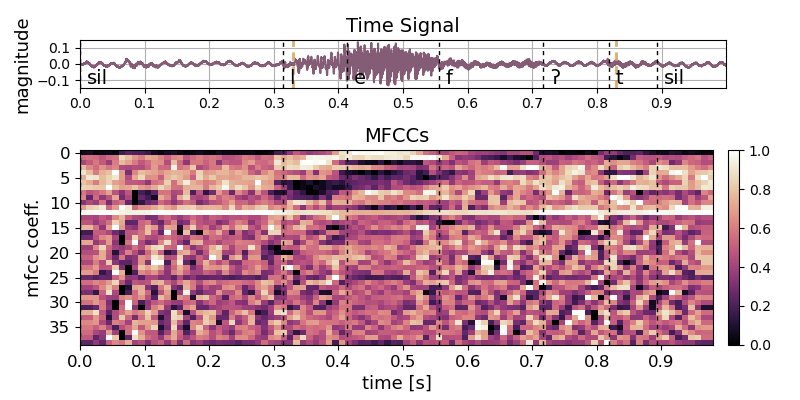
\includegraphics[width=0.45\textwidth]{./3_signal/figs/signal_mfcc_showcase_mfcc39_left0}}
    \subfigure[right]{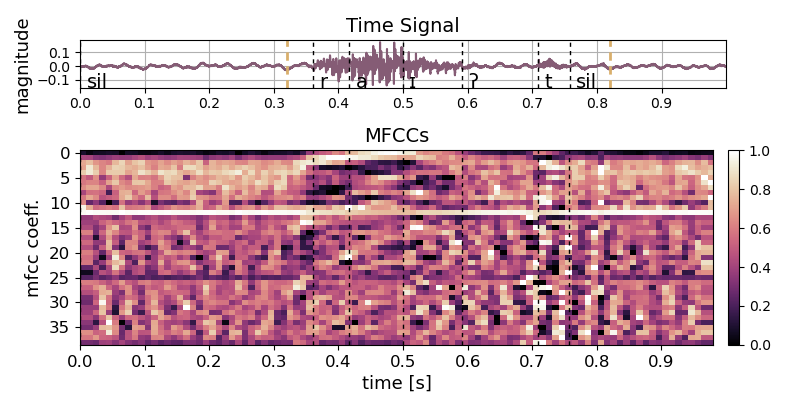
\includegraphics[width=0.45\textwidth]{./3_signal/figs/signal_mfcc_showcase_mfcc39_right0}}
    \subfigure[up]{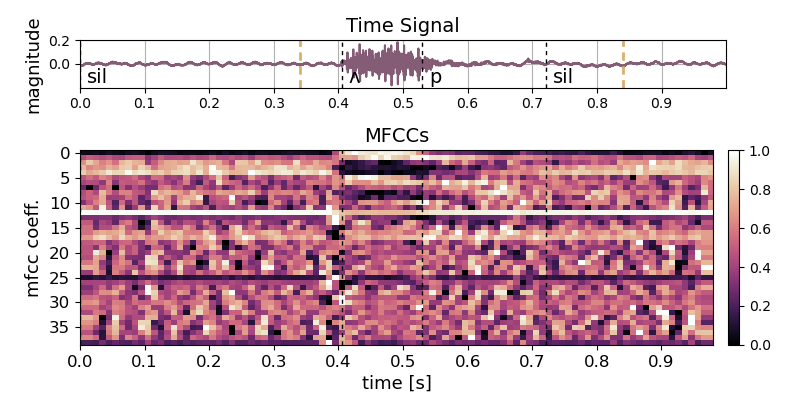
\includegraphics[width=0.45\textwidth]{./3_signal/figs/signal_mfcc_showcase_mfcc39_up0}}
    \subfigure[down]{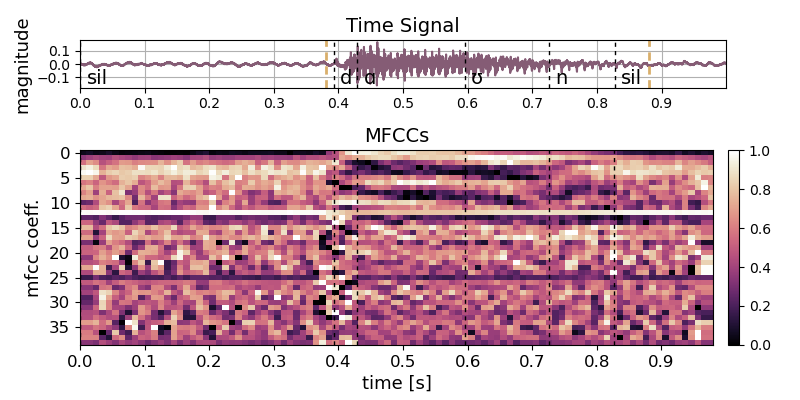
\includegraphics[width=0.45\textwidth]{./3_signal/figs/signal_mfcc_showcase_mfcc39_down0}}
    \subfigure[go]{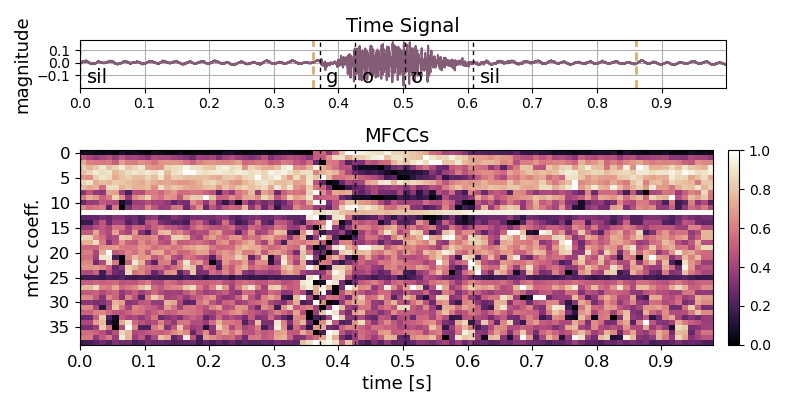
\includegraphics[width=0.45\textwidth]{./3_signal/figs/signal_mfcc_showcase_mfcc39_go0}}
  \caption{MFCC with 32 filter bands and 12 cepstral coefficients, deltas, double deltas and energy vector visualized with frame-based normalization.}
  \label{fig:signal_mfcc_showcase_mfcc39}
\end{figure}
\FloatBarrier
\noindent


% --
% energy consumption

\subsection{Computational Complexity}
The computational complexity is evaluated on the total amount of operations needed for a specific computation task, such as the feature extraction task of MFCCs.
The energy consumption is related to the computational complexity, but it is much harder to define and depends on many small parameters and actual hardware implementations, which is especially important for handheld devices.
The count of operations is sufficient for this thesis and provides a comparison to the benchmark models mentioned in \rsec{prev_kws_benchmark}.
The computational complexity for the computation of MFCC features are the amount of operations needed to process a \SI{1}{\second} time signal sampled with $f_s = \SI{16}{\kilo\hertz}$.
All MFCC specific extraction details are collected in \rtab{signal_mfcc_extraction_params}.
\begin{table}[ht!]
\small
\begin{center}
\caption{Parameters for determining the computational complexity of the MFCC feature extraction process.}
\begin{tabular}{ M{7cm}  M{2.5cm} M{2.5cm}}
\toprule
\textbf{Parameter} & \textbf{Value} & \textbf{Sample Length} \\
\midrule
Length of a signal $n$ & \SI{1}{\second} & 16000 \\
Analytic window size $N$ & \SI{25}{\milli\second} & 400 \\
Hop size $h$ & \SI{10}{\milli\second} & 160\\
\midrule
Fourier coefficients $K$ & 400  & - \\
Number of filter bands $B$ & 32 & -\\
Number of cepstral coefficients $C$ & 12 & -\\
\bottomrule
\label{tab:signal_mfcc_extraction_params}
\end{tabular}
\end{center}
\vspace{-4mm}
\end{table}
\FloatBarrier
\noindent
The amount of operations are the total number of additions and multiplications necessary to fulfill the process.
The major components of the MFCC are, as described in \rsec{signal_mfcc_pipeline} and summarized in \req{signal_mfcc_mfcc}, the transformation to the STFT, the weighting with the filter bands and the DCT transform.
The most costly component is of course the STFT, which again is composed of DFTs.
Note that the DFT uses complex multiplications and additions.
One complex multiplication equals to 4 real multiplication and 2 additions, so one complex multiplication consists of 6 operations.
For one complex addition, two real additions are necessary and equals therefore to 2 operations.
A general matrix multiplication with a vector $y = Ax$ where $A \in \R^{m \times n}$ and $x \in \R^n$ is composed of $m \cdot n$ multiplications and $m \cdot (n - 1)$ additions, where for simplicity the amount of additions is also assumed to be $m \cdot n$.

The amount of operations, denoted as $\mathcal{T(.)}$, for a trivial DFT transform with operator $\mathcal{F} \in \C^{N \times K}$ with $K$ Fourier coefficients on a windowed signal $x \in \R^N$ with sample length $N$ is:
% \begin{equation}
%   \mathcal{O}(x\mathcal{F}) = N \times K
% \end{equation}
\begin{equation}
  \mathcal{T}(x^T \mathcal{F}) = 6 (N K) + 2 (N K)
\end{equation}
and give for $N = K = 400$ the amount of operations $\mathcal{T}(x\mathcal{F}) = \SI{1.28}{\mega\ops}$ for a single DFT.
This of course are a lot of operations, luckily a more sophisticated Fourier transform can be applied with the Fast Fourier Transform (FFT) method, which gives a linear complexity and operations are calculated as:
\begin{equation}
  \mathcal{T}(x^T \mathcal{F}) = 6 (\mathcal{O}(N \cdot \log N)) + 2 (\mathcal{O}(N \cdot \log N))
\end{equation}
with $N = K = 400$.
The FFT has therefore roughly $\mathcal{T}(x^T \mathcal{F}) = \SI{20}{\kilo\ops}$ and is a huge improvement to the trivial method.
Further the interesting part of a DFT or FFT is only the half-band, because of the mirroring effect, which likewise may decrease the operations by half, so let the calculations be continued with Fourier coefficients of $K = 201$ of a half band and roughly $\SI{10}{\kilo\ops}$ per FFT.
The DFT is computed $M$ times, where $M$ is the total number of possible shifts calculated in \req{signal_spec_hop}, which gives with the evaluated parameters $M = 98$ frames.
So for the whole STFT $M$ is multiplied with the number of operations of each DFT, which give approximately $\mathcal{T}(\tilde{X}) = \SI{1}{\mega\ops}$.

The computation to the power spectrum and the log scaling are disregarded, so that two matrix multiplications remain:
$\abs{\tilde{X}}^2 \, W_m^T$ is a matrix multiplication of $\R^{M \times K}$ and $\R^{K \times B}$ which has $M K B$ real multiplications and approximately $M K B$ real additions, which give about $2 M K B = 2 \cdot 98 \cdot 201 \cdot 32 =  \SI{1.26}{\mega\ops}$.
The resulting band weighted STFT matrix $\R^{M \times B}$ is further multiplied with the DCT operator representing a matrix of $\R^{B \times C}$, that gives $2 M B C = 2 \cdot 98 \cdot 32 \cdot 12 = \SI{75}{\kilo\ops}$.
Altogether the matrix multiplications are approximately $\SI{1.26}{\mega\ops} + \SI{75}{\kilo\ops} = \SI{1.34}{\mega\ops}$.

The summary of the estimated operations are listed in \rtab{signal_mfcc_operations}.
% --
% mfcc operations
\begin{table}[ht!]
\begin{center}
\caption{Approximated number operations needed to transform a \SI{1}{s} time signal to MFCCs with parameters listed in \rtab{signal_mfcc_extraction_params}.}
\begin{tabular}{ M{6cm}  M{4cm}}
\toprule
\textbf{Process} & \textbf{Approximated Number of Operations} \\
\midrule
Power spectrum & \SI{2.71}{\mega\ops}\\
Weighting with equidistant Mel bands & \SI{1.26}{\mega\ops}\\
DCT transform of the weighted power spectrum & \SI{75}{\kilo\ops}\\
\midrule
\textbf{Sum} & \SI{4.05}{\mega\ops}\\
\bottomrule
\label{tab:signal_mfcc_operations}
\end{tabular}
\end{center}
\vspace{-4mm}
\end{table}
\FloatBarrier
\noindent


% --
% critism

\subsection{Criticism}
\thesisStateNew
MFCC are widely used for speech recognition tasks and perform very well, however the processing pipeline of MFCC has some disadvantages.
One disadvantage is, as already mentioned, that MFCCs are not intended for visualization, because of their broad value space of individual MFCC coefficients.
Another disadvantage is, that MFCC are not directly invertible to raw audio samples, because of the computation of the spectrogram.
Some inversion techniques exist \cite{Boucheron2008}, but it is still a rough approximation.
The inversion of MFCC would have been very interesting, when applied to generative neural networks, such as Generative Adversarial Neural Networks (GAN).



% --
% visualization

%\subsection{Visualization of MFCC features}\label{sec:signal_mfcc_visualization}


%To show this difference in value space in a negative example in practice, the MFCCs of the self-recorded speech command waveform \enquote{left0.wav} is shown in \rfig{left0_mfcc_only}.
% useless
% \begin{figure}[!ht]
%   \centering
%     \includegraphics[width=0.75\textwidth]{./3_signal/figs/signal_mfcc_left0_mfcc_only.png}
%   \caption{Bad visualisation of the 12 MFCCs features extracted from \enquote{left0.wav}.}
%   \label{fig:left0_mfcc_only}
% \end{figure}
% \FloatBarrier
% \noindent
% Not much structure of the MFCCs can be seen here, due to the vast value difference of the first coefficient. At least the first coefficient shows, where the center of signal energy is placed on the time scale, but other than that, this visualisation is worthless.
% Another very bad visualisation is shown by computing the 39 MFCC feature vectors (with Deltas, Double Deltas and Energies) in \rfig{left0_no_order}.

% \begin{figure}[!ht]
%   \centering
%     \includegraphics[width=0.75\textwidth]{./3_signal/figs/signal_mfcc_left0_no_order_norm0.png}
%   \caption{Very bad visualisation of 39 MFCC features extracted from \enquote{left0.wav}.}
%   \label{fig:left0_no_order}
% \end{figure}
% \FloatBarrier
% \noindent
% There appears an even greater gap of different value spaces and even less is seen.

% One solution is to show the features in different value groups. 
% For instance putting the first coefficient and its deltas is in one group, the other coefficients in another and their deltas and energies as well in own groups. 
% Now it is possible to observe some structure in the visualizations, with an example shown in \rfig{left0_order}.

% \begin{figure}[!ht]
%   \centering
%     \includegraphics[width=0.75\textwidth]{./3_signal/figs/signal_mfcc_left0_norm0.png}
%   \caption{Good visualisation of 39 MFCC features extracted from \enquote{left0.wav} with own value groupings.}
%   \label{fig:left0_order}
% \end{figure}
% \FloatBarrier
% \noindent
% Another way to improve the visualization is to normalize the feature vectors over each frame dimension with the infinity norm as:

% % frame normalisation
% \begin{equation}\label{eq:signal_mfcc_norm}
%   \hat{U}[m, l] = \frac{U[m, l]}{\norm{u_l[m]}_\infty}
% \end{equation}
% where $m$ is again the variable in frames, $l$ the individual MFCC coefficient and $u_l[m]$ the individual MFCC coefficient vector over all frames.
% This equation gives a value space between $[0, 1]$ for each feature vector $u_l[m]$.

% A visualization with frame normalization of the 39 MFCC feature vectors of \enquote{left0.wav} is shown in \rfig{left0_order},

% \begin{figure}[!ht]
%   \centering
%     \includegraphics[width=0.75\textwidth]{./3_signal/figs/signal_mfcc_left0_no_order_norm1.png}
%   \caption{Normalization of 39 MFCC features extracted from \enquote{left0.wav}.}
%   \label{fig:left0_no_order_norm1}
% \end{figure}
% \FloatBarrier
% \noindent
% or in an even better one shown in \rfig{left0_order_norm1}.

% \begin{figure}[!ht]
%   \centering
%     \includegraphics[width=0.75\textwidth]{./3_signal/figs/signal_mfcc_left0_order_norm1.png}
%   \caption{Normalisation of 39 MFCC features extracted from \enquote{left0.wav} with groups.}
%   \label{fig:left0_order_norm1}
% \end{figure}
% \FloatBarrier
% \noindent

% --
% onset

\section{Onset Detection}\label{sec:signal_onset}
\thesisStateReady
\thesisStateNew
Onset detection of key words is an essential part in Key Word Spotting (KWS) systems and describes the starting time of an actual key word.
In this thesis the onset detection is separated into:
\begin{itemize}
  \item key word onset detection (within a fixed time span)
  \item online onset detection
\end{itemize}
the key word onset detection is performed on already extracted time signals, such as raw data examples from the dataset, where the time interval of those signals are limited to \SI{1}{\second}.
The online onset detection runs during the recording of potential key words from a microphone input in a real time system.
Note that onset detection can be quite challenging and is of some sorts an own research subject.
For this thesis, however it is enough to use trivial methods, that do not use much computational effort.


% --
% key word onset detection

\subsection{Key Word Onset Detection}\label{sec:signal_onset_kw}
An intuitive method to detect the onsets of key words in a fixed time signal, is to simply use the signal energy.
Consider a fixed time signal $\bm{x} \in \R^n$ with a total number of $n$ samples, that is windowed with a striding frame of sample length $N$ corresponding to a time duration of \SI{500}{\milli\second}, the energy of each windowed signal is calculated as:
\begin{equation}\label{eq:e_win}
  e[m] = \sum_{i=0}^{N-1} \abs{x[m + i]}^2
\end{equation}
with shift index $m \in \mathcal{M} = \{0, 1, \dots, n - N + 1\}$.
The onset sample number $o \in \mathcal{M}$ with the highest energy region can be determined by
\begin{equation}\label{eq:onset}
  o = \underset{m \in \mathcal{M}}{\arg \max} \, e[m]
\end{equation}
for all windowed signal energies $e[m]$.
Note that it is assumed, that most of the key word in each signal is captured by the window length $N$ and that no noise peaks are present before and after the key word, otherwise the onset $o$ is shifted to either the left or right-hand side of the actual key word onset.
It is for sure, that this onset detection is not the most reliable one, but it is the simplest and most energy efficient method performed on raw audio data.

A better approach is to use energy values from the frequency response of the signal.
Since the Mel Frequency Cepstral Coefficients (MFCC) are extracted to obtain features for neural networks, it is straight forward to use them for onset detection as well.
The first cepstral coefficient $\bm{u}_0 \in \R^M$ of the MFCCs is actually an energy value, that is the sum of all equidistant mel filter bands.
The equivalent of \req{e_win} for MFCCs in the cepstral and frame space is therefore:
\begin{equation}
  e[m] = \sum_{i=0}^{N-1} \bm{u}_0[m + i]
\end{equation}
where $m$ and $N$ are in the frame space instead of the sample space.
A conversion from sample to frame space can simply be done by dividing the sample variable with the hop size $h$ in samples and rounding it to an integer number.
The onset frame $o$, using the first MFCC coefficient, is determined in the same way as formulated in \req{onset}.
An illustration of the onset detection with the fixed window of size \SI{500}{\milli\second} is shown in \rfig{signal_onset_window}, where
the start of the striding window with the highest energy value contained in this window, is the onset.
\begin{figure}[!ht]
  \centering
    
\includegraphics[width=0.55\textwidth]{./3_signal/figs/signal_onset_window}
  \caption{Striding window length of \SI{500}{\milli\second} used for energy calculation in onset detection.}
  \label{fig:signal_onset_window}
\end{figure}
\FloatBarrier
\noindent
A showcase on the performance of both energy onset detection methods are shown in \rfig{signal_onset_showcase}.
\begin{figure}[!ht]
  \centering
    \subfigure[left]{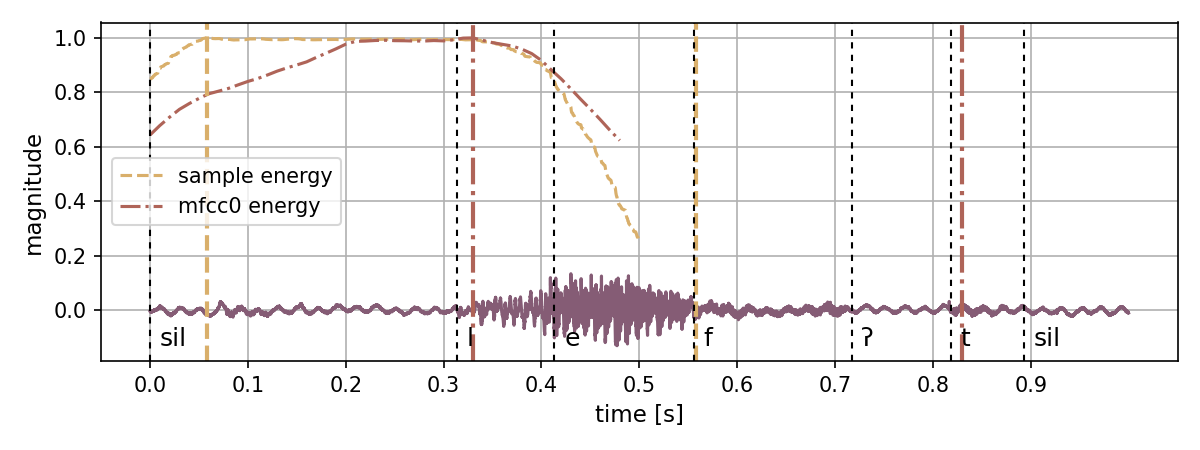
\includegraphics[width=0.45\textwidth]{./3_signal/figs/signal_onset_showcase_left0}}
    \subfigure[right]{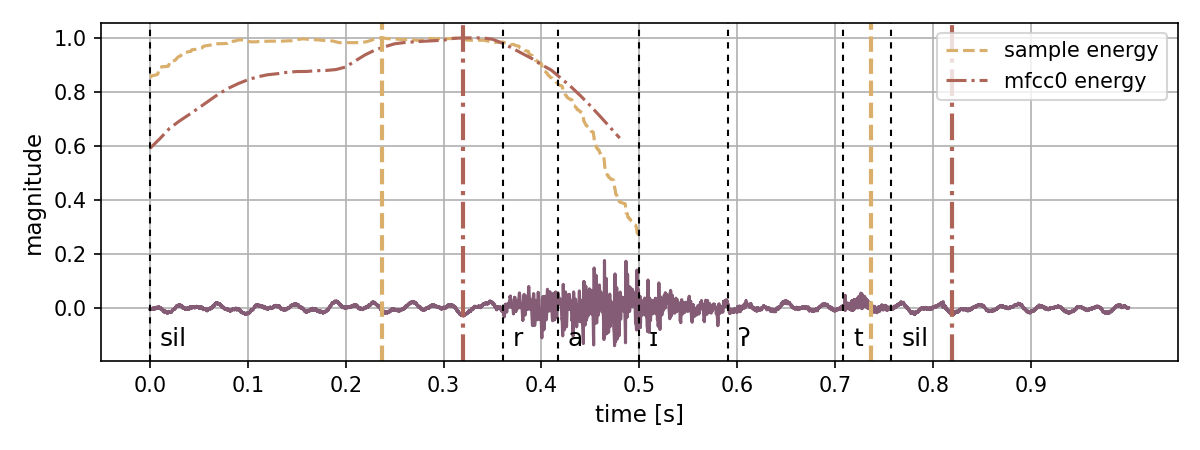
\includegraphics[width=0.45\textwidth]{./3_signal/figs/signal_onset_showcase_right0}}
    \subfigure[up]{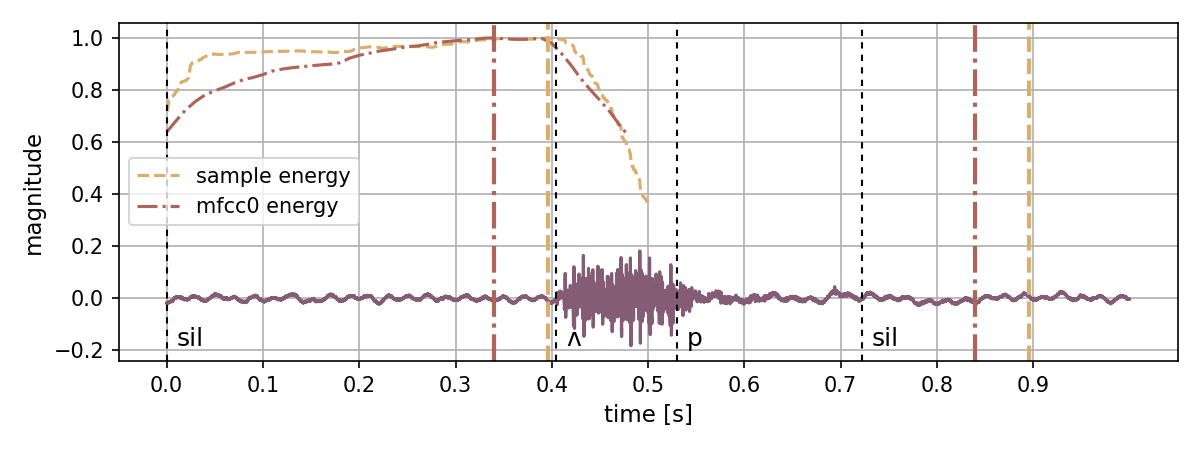
\includegraphics[width=0.45\textwidth]{./3_signal/figs/signal_onset_showcase_up0}}
    \subfigure[down]{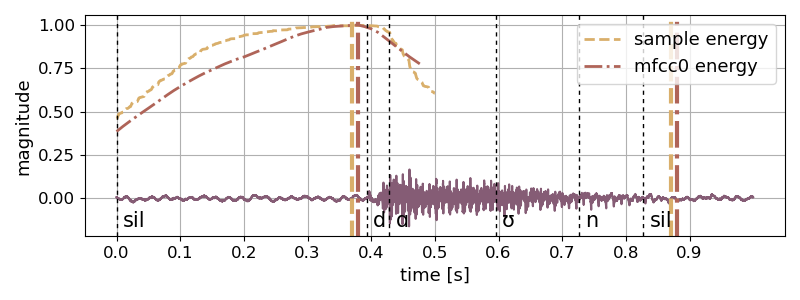
\includegraphics[width=0.45\textwidth]{./3_signal/figs/signal_onset_showcase_down0}}
    \subfigure[go]{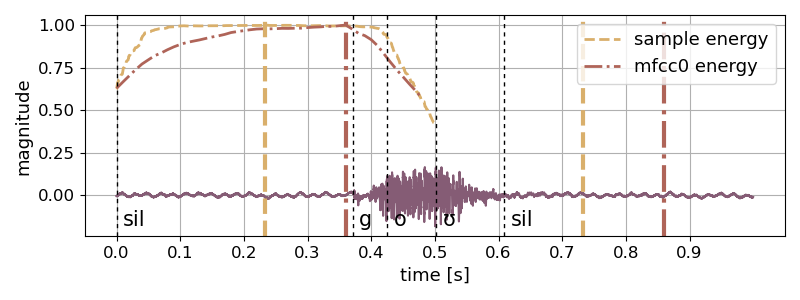
\includegraphics[width=0.45\textwidth]{./3_signal/figs/signal_onset_showcase_go0}}
  \caption{Onsets (vertical colored lines) obtained from the maximum of either the sample energy or first MFCC coefficient energy, with an analytical window length of \SI{500}{\milli\second}.}
  \label{fig:signal_onset_showcase}
\end{figure}
\FloatBarrier
\noindent
It can be observed that the MFCC onset method works much better, especially for the \enquote{left} example, where a little noise peak shifts the sample energy onset too far to the left so that the whole word is not captured.
For all MFCC extractions from the datasets during the experiments, the MFCC onset method is used. 
For raw audio extraction, applied in Wavenets, the sample energy method is applied.


% --
% key word onset detection

\subsection{Online Onset Detection}\label{sec:signal_onset_online}
The onset detection of online speech signals received from a microphone input stream, is processed by evaluating consecutive input chunks, that are stored in an input buffer.
From those input chunks the energy level can be computed and compared with an energy threshold, that should indicate the presence of an onset.
It is not the purpose to detect key word onsets by its correct starting time, but to signalize that a signal with enough energy is available for a potential key word classification.
Mathematically the onset $o(\bm{x}) \in \{0, 1\}$ of an input chunk $\bm{x} \in \R^n$ from an actual microphone input stream, can be obtained by:
\begin{equation}
  o(\bm{x}) = 
  \begin{cases}
    1, & \text{if } \frac{1}{n} \bm{x}^T \bm{x} > \alpha\\
    0, & \text{otherwise} 
  \end{cases}
\end{equation}
where the output value of $1$ represents the occurance of an onset, $n$ is the total sample number of the input chunk and $\alpha$ the energy threshold.
The energy threshold should be adjustable to the users microphone and ampliefier setup. 
This can be done for instance in the video game option menu as described in \rsec{game_interactables_menu}.
If an online onset is detected, the whole buffer is filled up first, then read and MFCC features extracted.
From those MFCCs the exact key word onset is calculated as described in \rsec{signal_onset_kw} and the \SI{500}{\milli\second} long feature vectors are sent to the classification system.
